\documentclass[border=5pt, tikz]{standalone}
\usetikzlibrary{perspective}
\usetikzlibrary{calc}
\usetikzlibrary{shadings}
\usepackage{amsmath}
\usetikzlibrary {arrows.meta,bending,positioning}
\begin{document}
 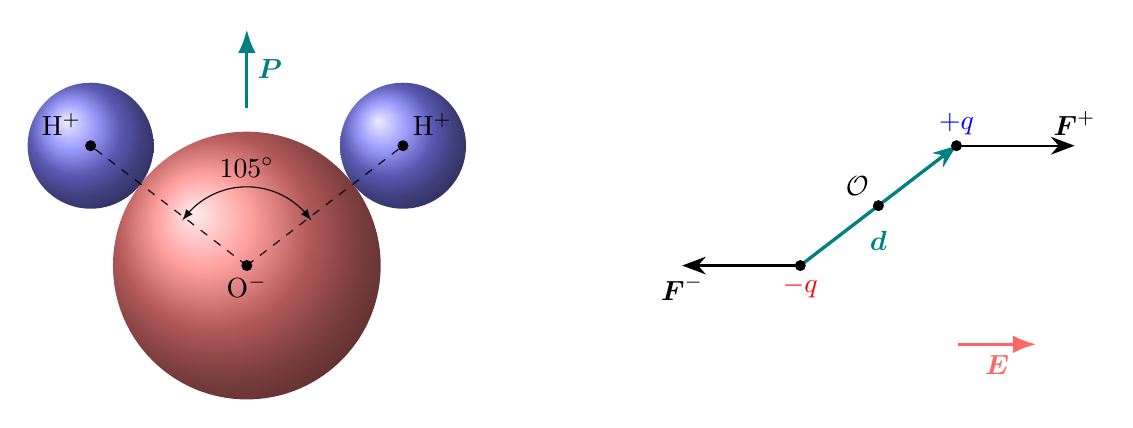
\begin{tikzpicture}

    \begin{scope}
        \coordinate (O) at (0, 0);
        \coordinate (H1) at ($(O) + (142.5:25mm)$);
        \coordinate (H2) at ($(O) + (37.5:25mm)$);

        \shade[ball color=red!50] (O) circle (17mm);
        \shade[ball color=blue!50] (H1) circle (8mm);
        \shade[ball color=blue!50] (H2) circle (8mm);
        \fill[] (O) circle (0.7mm);
        \fill[] (H1) circle (0.7mm);
        \fill[] (H2) circle (0.7mm);

        \draw[dashed] (O) node[below]{O$^-$} -- (H1) node [above left] {H$^+$};
        \draw[dashed] (O) -- (H2) node[above right] {H$^+$};

        \draw [latex-latex](35:10mm) arc (35:145:10mm) node [midway, above] {$105^\circ$};

        \draw [-{Latex[length=3mm]}, very thick, teal] (0, 20mm) -- (0, 30mm) node [midway, right] {$\boldsymbol{P}$}; 
    \end{scope}

    \begin{scope}[xshift=200]
        \coordinate (O) at ($(0, 0)+ (37.5:12.5mm)$);
        \coordinate (P1) at ($(0, 0) + (37.5:25mm)$);
        \coordinate (P2) at (0, 0);

        \draw [-{Stealth[length=3mm]}, very thick, teal] (P2) node [below, red] {$-q$} -- (P1) node [above, blue] {$+q$};
        \node [teal, below, yshift = -2mm] at (O) {$\boldsymbol{d}$};
        \fill[] (O) circle (0.7mm) node [above left] {$\mathcal{O}$};
        \fill[] (P1) circle (0.7mm);
        \fill[] (P2) circle (0.7mm);

        \draw [-{Stealth[length=3mm]}, thick] (P1) -- ($(P1)+(360:15mm)$) node [above] {$\boldsymbol{F}^+$};
        \draw [-{Stealth[length=3mm]}, thick] (P2) -- ($(P2)+(180:15mm)$) node[below] {$\boldsymbol{F}^-$};
        
        \draw [-{Latex[length=3mm]}, very thick, color=red!60] (2, -1) -- (3, -1) node [midway, below] {$\boldsymbol{E}$};

    \end{scope}
\end{tikzpicture}
\end{document}